%\documentclass{report}
%\usepackage[T1]{fontenc}
%\usepackage[utf8]{inputenc}
%\usepackage[francais]{babel}
%\usepackage{amsmath}
%\usepackage{graphicx}
%\graphicspath{{Figures/}}
%\usepackage[backend=biber,style=authoryear,bibencoding=utf8]{biblatex}
%\usepackage[colorlinks,linkcolor=blue]{hyperref}
%\newcommand{\micro}{$\mathrm{\mu}$}
%
%\begin{document}

\chapter{Localisation de MRTF-A dans les cellules musculaires en réponse à une stimulation mécanique}

\section{À propos de la localisation de MRTF-A}

 Comme on l'a vu dans le chapitre qui lui est consacré, la localisation de MRTF-A dans la cellule est liée à la concentration disponible en monomères d'actine : lorsqu'il y a des monomères en excès, MRTF-A est cytoplasmique car son NLS est caché, au contraire lorsqu'il n'y a plus assez de monomères disponibles le NLS est accessible et MRTF-A est dans le noyau. 
 
 Cela nous fournit un moyen simple de visualiser l'activation de MRTF-A/SRF : observer en fluorescence la localisation de MRTF-A dans la cellule. 
 
 Dans un premier temps, les cellules exprimant MRTF-A GFP, la version fluorescente du gène MRTF-A, peuvent être classées en trois groupes : celles pour lesquelles on peut distinguer le noyau en noir (la fluorescence est plus importante dans le cytoplasme), qui seront appelées Cytoplasmiques, celles pour lesquelles on peut distinguer le noyau en vert, appelées Nucléaires, et celles pour lesquelles le noyau ne peut être distingué, appelées Homogènes, comme on peut le voir sur les exemples en figure  \ref{Exemples_CHN}.
 
 \begin{figure}
  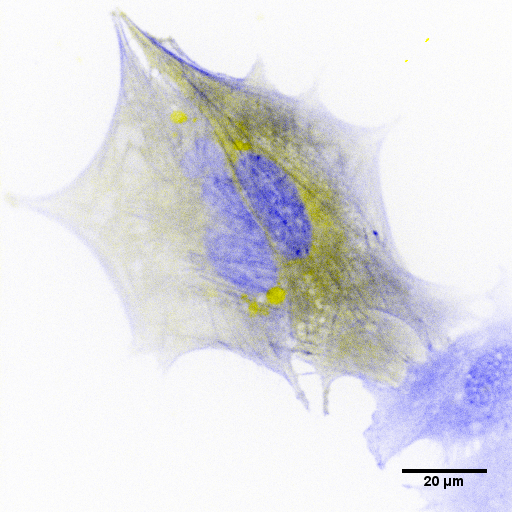
\includegraphics[width=3.5cm]{Figures/Exemple_C_invert.png} 
 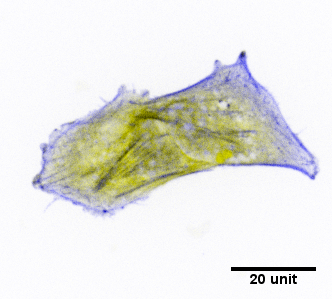
\includegraphics[width=3.5cm]{Figures/Exemple_H_invert.png} 
 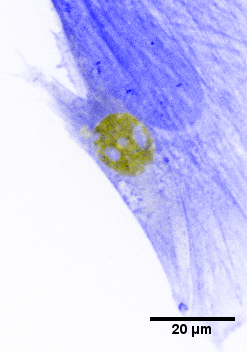
\includegraphics[width=3.5cm]{Figures/Exemple_N_invert.png} 
 \caption{Exemples de cellules classées comme MRTF-A Cytoplasmique, Homogène et Nucléaire, de gauche à droite respectivement. En bleu, la phalloïdine marquant les filaments d'actine, en jaune la MRTF-A GFP.\label{Exemples_CHN}}

 \end{figure}
 
 Dans un second temps, l'intensité de fluorescence dans le cytoplasme, dans le noyau et dans une zone péri-nucléaire a été mesurée quantitativement. Cette méthode est plus précise mais allonge considérablement le dépouillement. 
 Lorsque les images sont prises avec l'objectif 20X, nous ne prenons qu'un seul plan focal, mais il intègre le signal sur une certaine épaisseur de la cellule. Une zone épaisse, comme le noyau et la zone immédiatement autour, apparaîtra plus lumineuse en fluorescence qu'une zone fine comme un lamellipode, alors que la concentration en protéines est identique. 
 Pour comparer la concentration nucléaire à la concentration cytoplasmique, on remplace alors la mesure sur l'ensemble du cytoplasme par une mesure sur une zone autour du noyau qui a une épaisseur proche de celle du noyau. 
 On peut également comparer la totalité du signal dans le noyau à sa totalité dans le cytoplasme, car le rapport taille du noyau sur taille de la cellule est relativement bien conservé d'une cellule à l'autre. 
 
 

\subsection{Influence des moyens d'observation sur l'équilibre entre MRTF-A et l'actine G}

Les C2C12 ont été transfectées avec un plasmide contenant une copie du gène MRTF-A humain adjoint d'une séquence eGFP. 
Cela nous permet en microscopie d'observer quelle proportion de MRTF-A GFP se trouve dans le noyau, et quelle proportion dans le cytoplasme de la cellule. 
En revanche, au total, MRTF-A est sur-exprimée dans la cellule, en proportions variables d'une cellule à l'autre. 
Si MRTF-A est sur-exprimée en trop grande quantité, il ne reste pas assez de G-actine dans la cellule pour la maintenir dans le cytoplasme, et elle peut alors s'accumuler dans le noyau. 
Nous avons donc essayé de transfecter la quantité minimale de protéine nécessaire pour mener à bien les observations. 

On peut observer sur des cellules fixées et marquées avec l'anti-corps MRTF-A endogène qu'à l'état naturel, MRTF-A est toujours dans le cytoplasme de la cellule. 
Lorsque nous observons la MRTF-A GFP, ce n'est pas toujours le cas, et une proportion plus ou moins grande, selon la quantité de plasmide qui a pénétré les cellules, est contenue dans le noyau. 

L'objectif étant d'observer également le cytosquelette d'actine, nous avons mené des expériences avec un plasmide Actine mCherry, un plasmide LifeAct RFP, des marquages DNaseI et phalloïdine sur cellules fixées, et enfin avec de la siRactine, successivement.
 
L'ajout d'actine mCherry augmente le réservoir d'actine monomérique de la cellule, et d'autant plus que l'actine fluorescente polymérise un peu moins bien que l'actine sauvage, et donc participe à maintenir MRTF-A dans le cytoplasme. 
Cette méthode d'observation est donc loin d'être neutre pour notre système, comme on le verra plus loin.
 
La LifeAct est une petite protéine qui se lie aux filaments d'actine, et qui n'est pas censée interférer avec la polymérisation des filaments. Cependant, nous avons constaté une tendance à la stabilisation des filaments avec la LifeAct. De plus, sa fluorescence était trop intense et interférait de manière importante avec le signal de MRTF-A GFP. 

La DNaseI et la phalloïdine nous permettent d'observer à la fois l'actine F et l'actine G dans la cellule, mais ne peuvent être utilisées que sur des échantillons fixés, ce qui limite fortement l'observation de la dynamique de réorganisation du cytosquelette.
 
Enfin, la siRactine est une molécule nouvelle dérivée de l'association du jasplakinolide et d'une rhodamine, qui peut être utilisée en faibles concentrations \emph{in vivo} pour observer les filaments d'actine. 


\section{Application d'une force locale avec les pinces magnétiques}

Pour réaliser des expériences sur les cellules transfectées MRTF-A GFP, il a fallu monter les pinces magnétiques sous le microscope confocal. 
L'observation se faisait avec un objectif 40X à air, dans la géométrie à courte distance, ce qui nous permet d'appliquer localement de grandes forces (plusieurs centaines de pN) mais nous empêche d'observer suffisamment bien la position de la bille pour faire des mesures rhéologiques. 
Dans un premier temps, l'objectif était simplement de voir si l'application d'une force par les pinces magnétiques était suffisante pour déclencher une relocalisation de MRTF-A dans les cellules musculaires. 

Nous avons réalisé ces expériences sur trois séries de C2C12 : transfectées avec MRTF-A GFP seule (37 cellules observées), tranfectées avec MRTF-A GFP et une Actine mCherry (16 cellules observées), et transfectées avec MRTF-A GFP et le LifeAct RFP, qui marque les filaments d'actine dans les cellules vivantes (42 cellules observées, dont 34 témoins). 
L'objectf de ces doubles transfections était d'observer en même temps que la localisation de MRTF-A la réorganisation du cytosquelette. 

Parmi ces expériences, certaines cellules ont été observées alors qu'elles n'avaient pas de bille attachée à leur cytosquelette : ce sont des cellules témoins, sur lesquelles le champ magnétique a été appliqué comme pour les autres, mais sur lesquelles le champ n'est pas censé avoir un effet quelconque. 

\begin{figure}
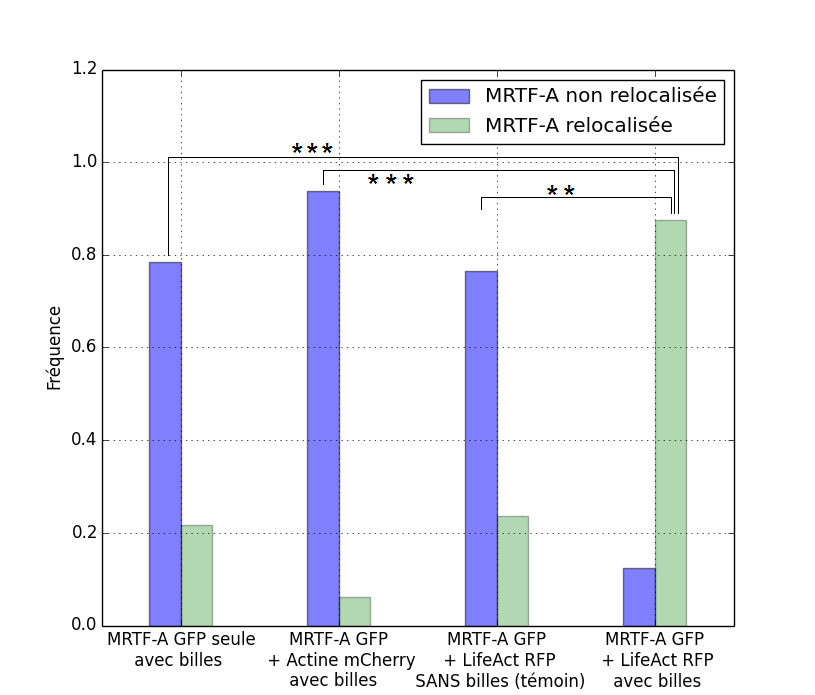
\includegraphics[scale=0.4]{Figures/Pinces_MRTFA_stars.png} 
\caption{Proportion des cellules observées pour lesquelles MRTF-A GFP change (en vert) ou ne change pas (en bleu) de localisation dans la cellule au cours de l'expérience. * : p<0.05 , ** p<0.01, *** p<0.001 (réalisés avec un test de Fisher)\label{MRTF-A Pinces}}
\end{figure}

On peut voir sur la figure \ref{MRTF-A Pinces} que l'ajout d'actine exogène réduit le nombre de cellules pour lesquelles MRTF-A change de localisation, mais de manière non significative, alors que l'ajout de Life Act RFP a l'effet inverse de manière significative. 
En effet, en ajoutant de l'actine mCherry, on augmente la quantité totale de G-actine dans la cellule, et ce d'autant plus que l'actine fluorescente polymérise un peu moins bien que l'actine sauvage. Comme plus de G-actine est disponible pour se lier à MRTF-A, celle-ci est d'autant plus susceptible d'être liée à l'actine et donc cytoplasmique. 
Si la réserve d'actine monomérique est grande, une polymérisation d'actine en réponse à la force appliquée ne sera pas forcément suffisante pour dépléter la réserve de G-actine excédentaire.

Au contraire, la LifeAct, en se liant aux filaments d'actine, peut les stabiliser en conformation polymérisée. En stabilisant la F-actine, la LifeAct rend donc la cellule beaucoup plus sensible à un recrutement de G-actine pour former de nouveaux filaments, et MRTF-A est plus susceptible de se retrouver sans liaison avec l'actine, et donc nucléaire.

De plus, on peut voir en comparant avec les expériences LifeAct témoin sans bille que l'application d'une force sur la cellule a un effet significatif sur la relocalisation de MRTF-A. 

On peut également remarquer que les résultats pour MRTF-A GFP seule sont identiques aux résultats avec LifeAct RFP mais sans application de force. 
On peut raisonnablement supposer que la force appliquée n'est pas suffisante ou n'est pas appliquée suffisamment longtemps pour réorganiser significativement le cytosquelette lors des expériences MRTF-A GFP seule, ce qui explique que leur activité soit proche des cellules témoins. 
La présence de Life-Act RFP stabilisant les filaments, la réserve d'actine monomérique est plus faible dans les cellules doublement transfectées MRTF-A GFP + LifeAct RFP, ce qui les rend plus sensibles : une contrainte plus faible suffit à dépléter suffisamment la réserve de G-actine. 

\begin{figure}
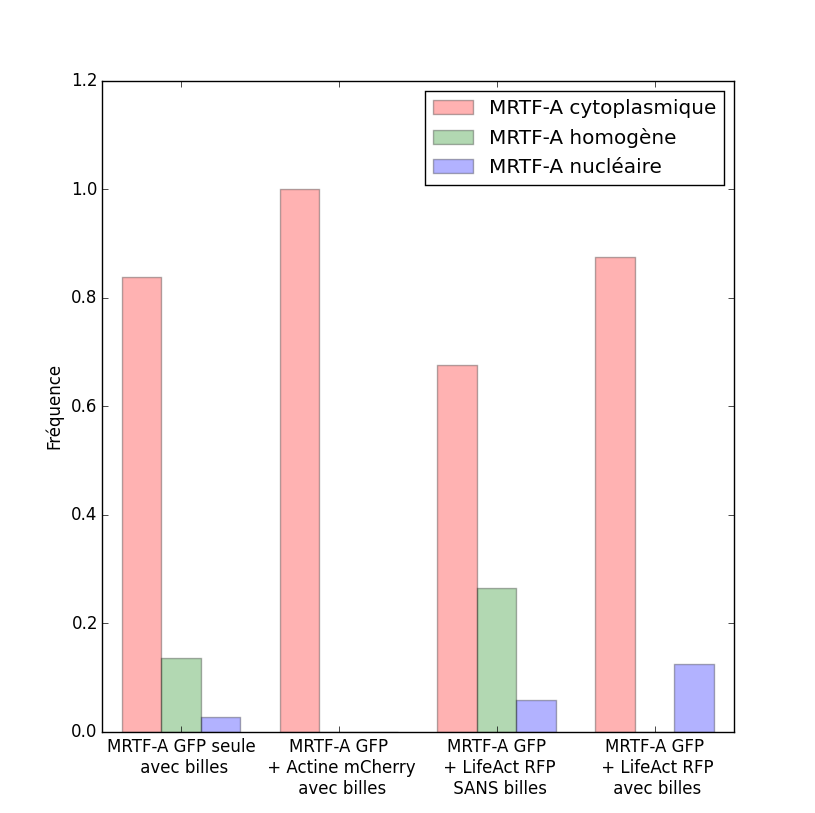
\includegraphics[scale=0.4]{Figures/CHN_pinces.png} 
\caption{Répartition de MRTF-A dans les cellules. \label{CHN_pinces}}
\end{figure}

On peut remarquer que la répartition de localisation de MRTF-A entre les différentes expériences est relativement semblable, ce qui implique que le changement d'activité observé sur la figure \ref{MRTF-A Pinces} n'est pas dû à l'état initial de MRTF-A dans ces cellules. 
Cependant, on peut noter une augmentation non significative de la quantité de cellules avec MRTF-A cytoplasmique avec l'actine mCherry, ce qui est cohérent avec la surexpression de l'actine, et une augmentation de la quantité de MRTF-A nucléaire avec la LifeAct, ce qui est également cohérent avec l'hypothèse d'une stabilisation des filaments par la LifeAct. 

\section{Application d'une déformation globale avec l'étireur : \'Etude qualitative et dynamique}

Les pinces magnétiques, lorsqu'il s'agit de suivre la dynamique sur une durée de l'ordre de la dizaine de minutes, ont l'inconvénient majeur de ne pouvoir opérer que sur une cellule à la fois. 
Il faut alors beaucoup de temps pour obtenir une population de taille acceptable avec cette méthode. 

C'est pourquoi les expériences sur MRTF-A ont été poursuivies par des déformations à l'aide d'un substrat étirable. De cette manière, on peut observer en général une trentaine de cellules pendant deux heures, là où précédemment on n'aurait pu observer que 4 cellules pendant 30 minutes. 



\subsection{\'Etat de référence}

\subsection{Effet de la surexpression d'actine mCherry}

\subsection{Effet du rinçage et du montage préalables}

En faisant des expériences témoin durant lesquelles aucun étirement n'était imposé, nous avons commencé à soupçonner qu'une ou plusieurs étapes de la préparation de l'échantillon pouvaient interférer avec les expériences. 
Deux étapes ont été testées : la première est l'étape durant laquelle on sort la lamelle de la plaque six puits pour la monter dans l'étireur, et qui implique des contraintes mécaniques sur la lamelle ; la seconde est l'étape de rinçage durant laquelle le milieu de culture des puits était remplacé par du milieu neuf dans l'étireur, ce qui pouvait induire une variation de la concentration en sérum. 

Pour l'étape de montage, nous avons testé le montage juste avant l'expérience (Montées), et le montage la veille au soir (Prémontées). 
Le rinçage est toujours effectué en même temps que le montage. 


\begin{figure}
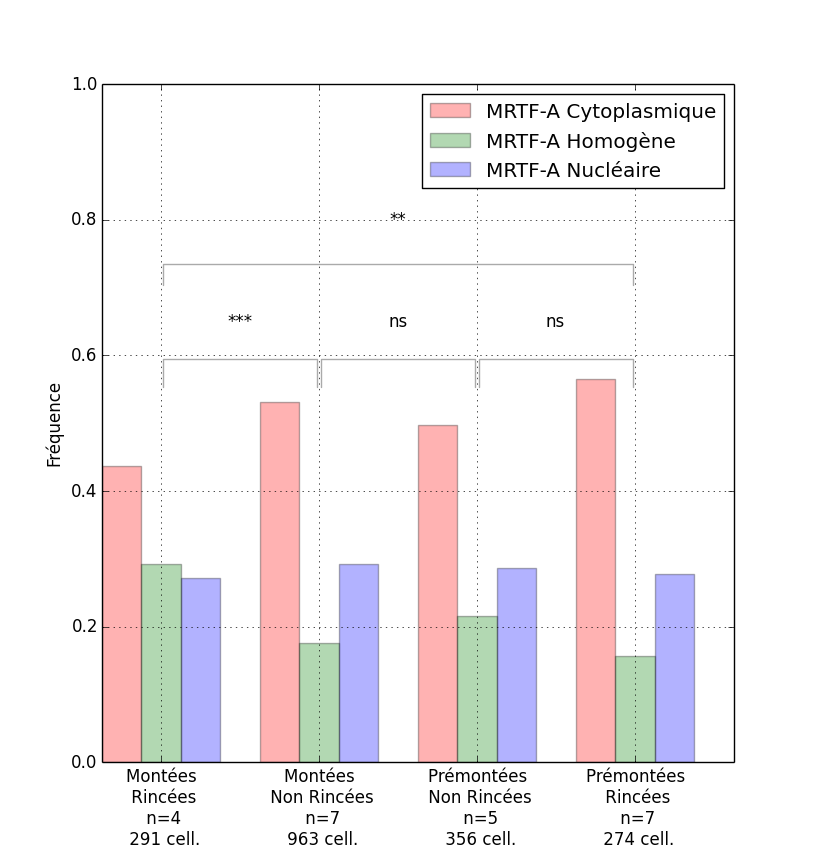
\includegraphics[scale=0.5]{Figures/CHN_montage_rincage.png} 
\caption{\label{CHN_montage} Influence sur la localisation de MRTF-A des contraintes mécaniques dues au montage de la lamelle dans l'étireur (Montage) et de la variation de concentration en sérum due au remplacement du milieu de culture par du milieu neuf au moment du montage (Rinçage). Montées : montage à $t-5$ minutes, Prémontées : montage à $t-18$ heures, rinçage au même moment.
Tous les tests on été réalisés avec un G-test d'indépendance t et une correction de Bonferroni pour les comparaisons multiples. ** : $p<\frac{0.01}{4}$ et *** : $p<\frac{0.001}{4}$}
\end{figure}

On peut voir sur la figure \ref{CHN_montage} que lorsque les cellules sont rincées juste avant l'expérience (Montées Rincées vs Montées Non Rincées), il y a significativement moins de cellules pour lesquelles MRTF-A est majoritairement cytoplasmique. 
Comme son nom l'indique, Serum Response Factor est puissamment activé par le sérum, et ici le seul rinçage avec du milieu neuf suffit à activer la voie de signalisation MRTF-A/SRF et changer la localisation de MRTF-A d'une partie des cellules. 
On également constater que lorsque le rinçage est effectué la veille (Prémontées Rincées vs Prémontées Non Rincées), il n'y a plus aucun effet. 

On peut également voir que l'étape du montage n'a pas la même influence selon qu'il y a rinçage ou non. Sans rinçage, cette étape n'a pas d'influence significative sur l'état des cellules, en revanche avec rinçage, on peut remarquer que le montage a tendance à augmenter la quantité de cellules ayant MRTF-A dans le cytoplasme au dépens de celles l'ayant réparti de manière homogène. 

Une fois ces résultats mis en évidence, nous avons réalisé la suite des expériences en évitant scrupuleusement de changer le milieu de culture dans lequel baignent les cellules le jour même de l'expérience. 

\subsection{Résultats pour l'étirement 10\%}

\subsection{Résultats pour l'étirement 30\%}

\section{Application d'une déformation globale avec l'étireur : \'Etude quantitative sur cellules fixées}

\subsection{Résultats pour l'étirement 10\%}

\subsection{Résultats pour l'étirement 30\%}

\section{Application d'une déformation globale avec l'étireur : \'Etude quantitative dynamique}












%
%\end{document}